\chapter{Relational Data Model \& Relational Algebra} % Depth 0

\section{RDBMS}

\begin{itemize}
    \item Database Management System (DBMS) : a computer system for creating and maintaining databases
    \item Relational Database Management System (RDBMS) : databases which consists of \textit{tables} (relations)
\end{itemize}

\begin{figure}[H]
    \centering
    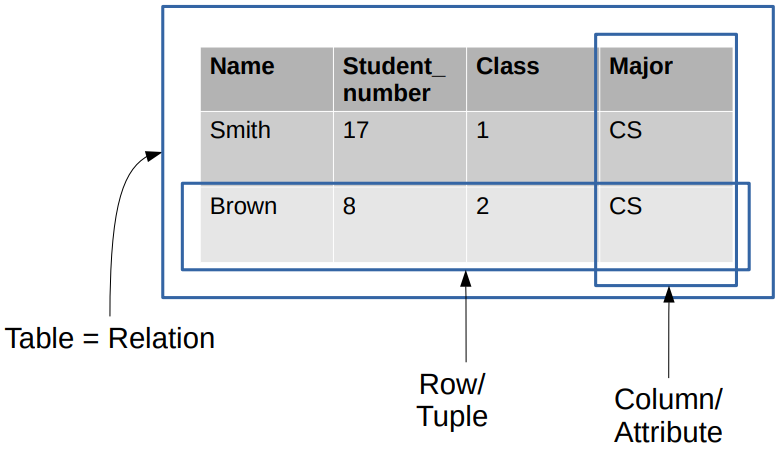
\includegraphics[width=0.6\textwidth,keepaspectratio]{RDBMS}
\end{figure}

\begin{Parallel}{0.47\textwidth}{0.47\textwidth}
\ParallelLText{
	\textgreen{\large{Pros}}
	\begin{itemize}
	    \item Ease of use due to abstraction (Logical/Physical independence)
	    \item Well known languages (SQL)
	    \item Reliability
	\end{itemize}
}

\ParallelRText{
	\textred{\large{Cons}}
	\begin{itemize}
	    \item Harder to obtain good performance, in particular in a distributed setting
	    \item Do not natively support very well some structures (Graph, Geographical data, Time-stamped data, ...)
	\end{itemize}
}
\ParallelPar
\end{Parallel}

\section{Relational Algebra}

Relational algebra is a set of mathematical rules and operators used to manipulate and query data in a relational database.

\subsection{Basic operators}

\begin{itemize}
    \item \textblue{Selection} $\sigma_{\text{(<selection condition>)}}(R)$ : used to denote the \textit{SELECT} operator. The \textit{selection condition} is a boolean expression specified on the attributes of relation \textit{R}.
        \begin{itemize}
            \item It is \textit{commutative} : $\sigma_{(\text{<cond1>)}}(\sigma_{(\text{<cond2>})}(R)) = \sigma_{(\text{<cond2>})}(\sigma_{(\text{<cond1>})}(R))$
            \item A cascade of selections can be combined : $\sigma_{(\text{<cond1>})}(\sigma_{(\text{<cond2>})}(...(\sigma_{(\text{<condn>})}(R))...)) =$ \\$\sigma_{\text{(<cond1> \textbf{AND} <cond2> \textbf{AND} ... \textbf{AND} <condn>})}(R)$
            \item In Rel : $\sigma_{(\text{Age}=20)}$(Student) = $\{t \in \text{Student} \ | \ t.\text{Age}=19 \}$
            \item In SQL : SELECT * FROM Student WHERE Age=20
        \end{itemize}
    \item \textblue{Projection} $\pi_{\text{<attributes>}}$ : selects a subset of columns from a table. The operation \textbf{removes any duplicate tuples}, so the result is a set of distinct tuples, and hence a valid relation (known as \textbf{duplicate elimination})
        \begin{itemize}
            \item In Rel : $\pi_{\text{Age}}$(Student) = $\{ t[\text{Age}] \ | \ t \in \text{Student} \}$
            \item In SQL : SELECT DISTINCT Age FROM Student
        \end{itemize}
\end{itemize}


